\section{Realisierung}
\subsection{Vorgehensweise}
Als Vorgehensweise wurde das erweiterte
Wasserfall-Modell gewählt. (Abbildung~\ref{fig:wasserfall_modell})
\begin{figure}[h]
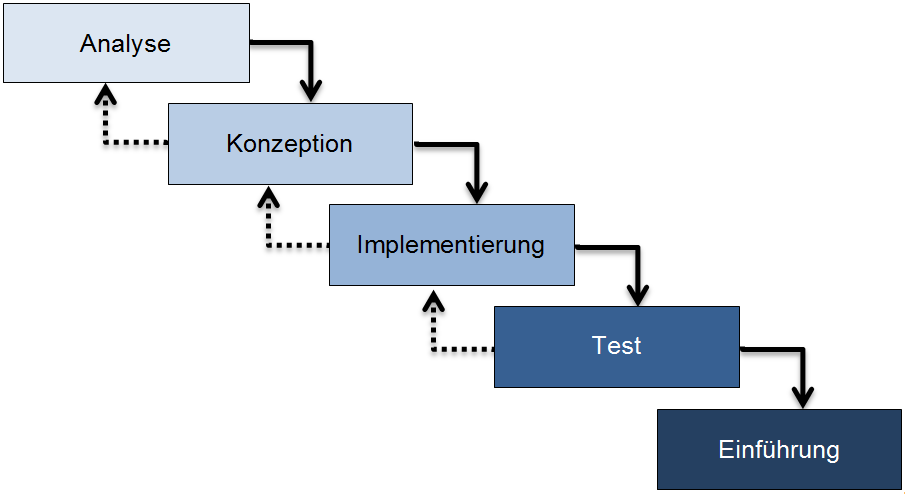
\includegraphics[scale=0.5]{img/wasserfall_modell.png}
\caption{Erweitertes Wasserfallmodell\label{fig:wasserfall_modell}}
\end{figure}
Aufgrund der knappen Zeitanforderungen bietet ein solcher Ansatz
den Vorteil eines direkten, klaren Pfades vom Beginn zum Ende des
Projektes. Im erweiterten Wasserfall-Modell erhält man, durch die
Möglichkeit kleine Rückschritte zu machen, die nötige Flexibilität um
auf Feedback einzugehen und Dinge ausprobieren zu können.
\subsection{Analyse \& Konzeption}
Bei der Analyse der Anforderungen fallen die Realtime Aspekte auf. Sie
sollen mithilfe von Websocketkommunikation und Push-Based-Updates vom
Server umgesetzt werden. Für einen modernen Look und ein intuitives
Verhalten soll die Steuerung Drag and Drop unterstützen.
\subsubsection*{Architektur}
Zu Beginn wurde ein Plan für das grobe Zusammenspiel der beteiligten
Komponenten angefertigt. Hiermit wurde die Arbeit in mehrere Schritte
und leicht abzugrenzende Komponenten unterteilt. Das Projekt ließ sich
damit in Meilensteine aufteilen, um strukturiert an das Projekt
herangehen zu können.

Die Architektur gibt dabei folgende Aufteilung her:
\begin{itemize}
\item Datenbank
\item Backend Server
\item Desktop Frontend
\item Mobile Frontend
\end{itemize}
Einen Überblick über die spätere ``physikalische Ausprägung'' des
Systems soll Abbildung~\ref{fig:architektur} geben.
\begin{figure}[h]
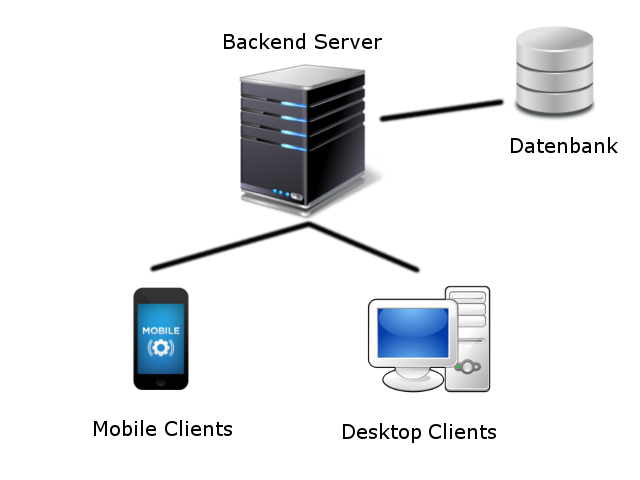
\includegraphics[scale=0.5]{img/Architektur.png}
\caption{Architektur Übersicht\label{fig:architektur}}
\end{figure}
Die Clients (Mobile / Desktop) kommunizieren über WebSockets mit dem
Backend-Server. Dieser speichert und liest Daten aus einer Datenbank.
Durch die WebSockets ist es dem Backend-Server möglich Änderungen am
Datenmodell mittels Push-Benachrichtigungen an die Clients weiterzugeben.
\subsection{Implementierung}
\subsubsection{Browser-Frontend}
Die Implementierung des Browser-Frontends verwendet Technologien, die
dem \gls{Reactive Programming} Pattern zuzuweisen sind. \gls{React} als
UI-Framework von Facebook ist ein stark durch funktionale Ideen und
\gls{Reactive Programming} inspiriertes Framework. Dies bedeutet
konkret, dass die elementaren Objekte der Programmierung keine
skalaren Werte wie Numbers oder Strings sondern Streams von
solchen sind. Dies erlaubt es, Werte die sich über die Zeit verändern,
in einem deklarativen Stil zu beschreiben und angemesssene
Abstraktionen für Echtzeitsysteme zu finden. \gls{Reactive
  Programming} ermöglicht außerdem besonders kurze Antwortzeiten auf
Nutzerinteraktion, was zu einem besseren Nutzererlebnis führt. Die
Applikation leidet nicht unter Ladezeiten und reagiert schnell und
zuverlässig.

Das Browser Frontend ist modular aufgebaut, wobei das Modulsystem von
\gls{PureScript} behilflich ist. Ein Modul kapselt dabei die
Definitionen innerhalb einer Datei und kann von anderen Modulen
importiert werden. Dies erlaubt es das Dateisystem zu nutzen um Teile
des Systems inhaltlich voneinander abzugrenzen. Das Prinzip von der
starken Kohäsion und losen Kopplung ist ein wichtiges Ziel bei der
Architektur und dem Design von Software und lässt sich mithilfe des
Modulsystems von PureScript leichter umsetzen.

Die Kommunikation mittels WebSockets und das Verwalten des
Applikationszustandes geschieht in der in \gls{PureScript}
implementierten Engine. Dieser Teil des Programmes nimmt im
Unidirectional-Dataflow Modell die Rolle der ``Stores'' ein und
erlaubt es das View-Layer beliebig auszutauschen. Die Engine ist für
alle Clients gleich und kann daher für die mobile Version des Clients
wiederverwendet werden.

\begin{figure}[h]
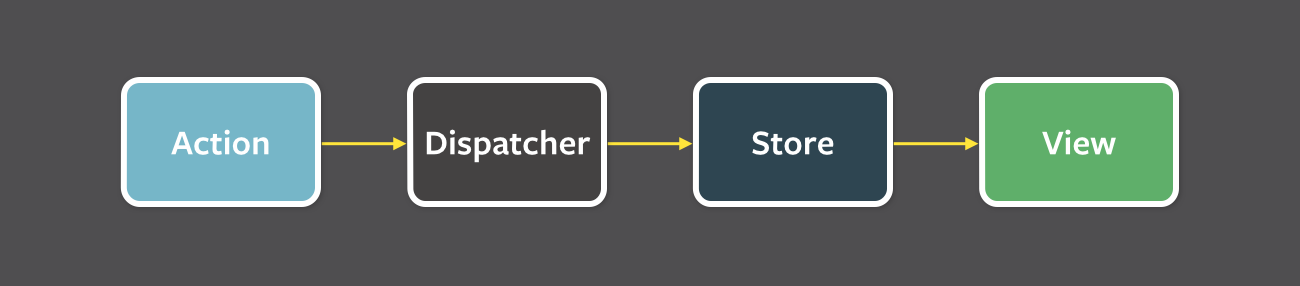
\includegraphics[scale=0.3]{img/Unidirectional.png}
\caption{Unidirectional Dataflow}
\end{figure}

\noindent Die Engine ``pusht'' den Applikationszustand in das
View-Layer, welches aus diesem ein User Interface rendert.
Die Interaktionen des Benutzers mit dem View-Layer erzeugen dann
wiederum Events, die als Streams an die Engine zurückfließen, wo sie
interpretiert und verarbeitet werden. Das Interpretieren der Events
lässt sich, dank des deklarativen Stils den PureScript erlaubt, leicht
programmieren. Als Beispiel soll der Code dienen, der das Ziehen eines
Themas auf das Grid beschreibt.

\begin{lstlisting}
  dragTopic = do
    Right t <- dragStart
    action <- dragOver
    lookup "dragEndTopic" `merge` lookup "dragEndGridTopic"
    return $ action t
\end{lstlisting}
\noindent Hier werden die Eventstreams für den Beginn eines
Drag Vorgangs sowie das Ziehen über einen Zeitslot mit dem Beenden des
Drag Vorgangs kombiniert und in einem resultierenden Stream \texttt{dragTopic}
ausgegeben. Dieser Stream abstrahiert nun die Mechanik des Drag and
Drop Vorganges und erlaubt es die tatsächlichen Intentionen des
Nutzers zu modellieren, um angemessen auf diese reagieren zu können.
\subsubsection{Backend Server}
Für die Entwicklung des Backend Servers wurde Haskell als
Programmiersprache ausgewählt. Haskell ist eine rein funktionale
Sprache und bringt dadurch die schon angesprochenen Vorteile im Bezug
auf Modularität und Skalierbarkeit mit sich. Die Implementierung
verwendet das \gls{Yesod Framework}, welches bereits Funktion für das
Ausliefern von HTML, CSS und JavaScript bereitstellt. Weiterhin erleichtert
das \texttt{Yesod.WebSockets} Modul das Programmieren der WebSocket
Endpunkte. Der Applikationszustand wird am Backend genau so wie auch
am Frontend laufend durch Events von Clients verändert. Anstatt jedoch
die Änderungen an die anderen Clients zu verteilen, werden die Events
per ``Broadcast'' Mechanismus verteilt. Jeder Client kann dann seinen
Applikationszustand selbst fortschreiten. Dies hat den Vorteil, dass
Clients, die für eine gewisse Zeit vom Netz getrennt waren, alle
``verpassten'' Events nachholen können und nicht ganz von vorne
beginnen müssen.
\subsection{Test \& Abnahme}
Der Client wurde auf verschiedenen Endgeräten getestet. Hierbei fielen
immer wieder Kleinigkeiten auf, die sich unterschieden. Das Beheben
dieser kleinen Bugs gestaltete sich als zu zeitaufwendig, und so wurden
die unterstützten Browser auf Firefox und Chrome festgelegt.
Die Mobile Version wurde sowohl auf Android als auch auf iOS ausgiebig
getestet und funktioniert ohne Einschränkungen auf beiden Systemen.
\subsection{Projektablauf}
Die folgende Tabelle soll die Differenzen zwischen \textit{Soll} und \textit{Ist} in
der Zeitplanung aufzeigen.
\begin{table}[htb]
\centering
\begin{tabular}{l l r r r}
\toprule
   & Phase                & Soll & Ist & Diff. \\
\midrule
1. & Planung              & 2h  &  2h & $\pm0$ \\
2. & Entwurf              & 5h  &  5h & $\pm0$ \\
\midrule
3.  & Implementierung     &     &     &        \\
3.1 & Browser Frontend    & 15h & 17h & $  +2$ \\
3.2 & Backend             & 20h & 15h & $  -5$ \\
3.3 & Mobile Webapp       & 5h  &  8h & $  +3$ \\
\midrule
4. & Abschließender Test  &  5h &  5h & $\pm0$ \\
5. & Übergabe             &  3h &  3h & $\pm0$ \\
6. & Dokumentation        & 15h & 15h & $\pm0$ \\
\cmidrule{3-5}
$\Sigma$ & Summe          & 70h & 70h & $\pm0$ \\
\bottomrule
\end{tabular}
\caption{Vergleich Aufwand -- Soll/Ist}
\end{table}

\noindent Die Zeitersparnis von 5 Stunden bei der Entwicklung des
Backends rührt daher, das durch die syntaktische und semantische Nähe
von PureScript und Haskell einiger Code mit wenigen Änderungen vom
Frontend übernommen werden konnte. Der Code der übernommen werden
konnte musste jedoch erst am Frontend entstehen, weshalb hier über das
erwartete Zeitbudget hinaus entwickelt werden musste.

\noindent Dass für die Mobile Webapp 3 Stunden mehr als ursprünglich
geplant aufgewendet werden musste, lag an den Inkompatibilitäten der
mobilen Browser untereinander. Hier mussten Änderungen gemacht und
mühsam auf vielen Geräten getestet werden.

Die Zeitplanung hat sich erfreulicherweise jedoch als akkurat
herausgestellt und so konnte das Projekt im gegebenen Zeitrahmen
realisiert werden.

%%% Local Variables:
%%% mode: latex
%%% TeX-master: "../Doku"
%%% End:
